% !TeX root = ../Thesis.tex
\chapter{Proof of Latency}
\label{Proof of Latency}
Proof of Latency, "the algorithm" or "PoL", is an algorithm that when used in a P2P context, can offer a robust way of reducing network latency between peers by minimizing the number of hops between peers that are close in terms of performance and geographical location. PoL also makes network bootstrapping faster, making it easier to find performant, close-by peers on first interaction with PoL-enabled network. PoL can result in a network in which a peer can estimate its latency to another peer before connecting to it.

The algorithm is trustless and requires no specific hardware from the participants, while a trusted computing platform would make it fairer and more reliable by not discriminating based on processing performance. An ASIC VDF chip would also make any of the later mentioned attack vectors less relevant by removing variance in hardware.

\section{Use Cases}
The section Peer-to-peer Networking described the problems Proof of Latency is trying to solve. While the use in P2P routing might be a no-brainer, the same algorithm can be used for computation performance benchmarking. In the next sections I will describe these use cases more thoroughly.

\subsection{Dynamic P2P Routing}
The use case that drove me to proceed working on Proof of Latency is an idea that there could be a trustless way of telling to other peers how much latency you have to another peer. In current P2P systems, if one peer were to tell you that it had a 10ms latency to another peer, there would be no quarantees of the 10ms latency holding true. If we could make a proof of that latency using cryptography, you could tell that the reported latency is true, and some work has been done to calculate it. This kind of proof could also make eclipse attacks harder to accomplish by requiring a closer distance or more resources to reach a lower latency to the targeted peer.

% TODO: Explain this idea WAAAAAY further

Although DHTs like Kademlia do peer distribution basically at random based on identifier closeness, there are no guarantees that when a peer connects to peers it has received from an another peer are also random, and thus the promise of random peer walk is lost. With Proof of Latency, you can be sure that the peers advertised are actually close-by. Of course, this is easily avoided by the attacker by spawning multiple peers in the same location.

\subsection{Benchmark Queries}
A protocol like this could be used to query for performance. In fact, Proof of Latency does that already, but processor development might render that property less effective in the future, unless one were to measure parallel processing capability with multiple VDFs, for example. Parallel multiple VDFs have been thought of and tested before, but calculating multiple separate VDFs has not been useful in previously imagined use cases, since it doesn't serve as a measure of time, but performance.

This could serve as a part of a greater protocol in a distributed computation system. It would be very unfortunate to run large datasets against a data analysis model on a mobile phone, and it could be beneficial to prove that the peer that advertises its services can actually run the computation without hiccups.
% TODO Cite?
There have been proposals for a VDF-as-a-function system, in which less performant peers could query for a VDF calculation if they don't have the means to do so in a time frame small enough themselves. The FPGA based system is being tested right now on Amazon Web Services cloud platform.~\{Devlin2020-qw} A benchmark query using PoL could also be a part of such a system to verify peers' ability to perform VDF calculations faster than the querying peer.

\section{Role of Latency in Distributed Systems}
It's hardly a surprise, but latency is a huge factor in distributed systems, especially trustless, decentralized ones. Latency is mostly constrained by the speed of light, which can not be changed, and thus there are concrete factors that must be taken into account when designing a P2P system with routing. In 2012, the global average round-trip delay time to Google's servers was around 100ms.~\cite{Grigorik_undated-mc}

In the new space age the maximum possible latency grows very fast, as there could be peers joining to a distributed network from other planets, space ships or stations. This might be unnecessary to think about in the distributed P2P context for now, but before all that, we have global satellite mesh internet providers, like Starlink. Elon Musk, the founder of SpaceX, which provides the network of satellites, claims that there's going to be a round-trip\footnote{Including the user's initial request and received response} latency of about 20 milliseconds between a single satellite and the user.~\cite{Tung_undated-ny} In legacy satellite internet access, the round-trip time even in perfect conditions is about 550 milliseconds.~\cite{noauthor_undated-zc} This difference between legacy and newer satellite internet comes from the difference in their orbits and the sheer amount of satellites involved. Legacy satellite internet uses geostationary orbits, which are very high, beaming on a single face of the earth at a time with limited bandwidth. Newer systems, like Starlink, use a low-earth-orbit, which requires more satellites, since they zoom by at such a speed that constantly changing which satellite you're connected to is a must. The low orbit also means less distance between the satellites and the user. The 20 millisecond latency claimed by Starlink at first seems like a stretch, but is believable when you take into account that inter-satellite links are done by laser, and light can travel about 31 percent faster in a vacuum than in fiber optics.~\cite{Finley2013-wt} Intercontinental latencies can become much lower because of this.
In blockchains, latency plays a role in the efficiency of the power used to achieve consensus. Miners waste energy on a previous block as long as they don't receive information on the winner of the previous block race. Simulations by Wei Bi, Huawei Yang, and Maolin Zheng in their paper An Accellerated Method for Message Propagation in Blockchain Networks have shown that if you calculate the round-trip time between the peers that are connected to each other and dropping the ones with larger latencies in favor of lower ones, you can achieve 50\% improvement in average latency with 1 to 2 peers connected. When connectedness grows from the degree of just 1-2 peers up to 20 connected peers, the average latency improvements achieved drop to about 20\%.~\cite{Bi_undated-is} You can't keep multiplexing connections\footnote{Having multiple concurrent stateful connections.} forever, though, and there's a Goldilocks zone for the most effective amount of connections. When connectedness increases, there's shorter routes simply by chance to peers you're not directly connected to, and protocols like publish-subscribe schemes work faster, propagating their messages to the whole network faster because there's less relaying happening. There are hardware and software related limitations to the amount of peers. On IPFS, for example, the protocol has been breaking user's routers~\cite{Whyrusleeping2016-ej} because of the high number of incoming connections that need to be routed through NAT\footnote{Network address translation. Hides the local area network from the internet under a different subnet address.}.

\section{Network Hops Increase Latency}
Network hops in P2P systems are introduced when two peers are not directly connected to each other, but rather through one or many relays. There are network hops that cannot be easily avoided, like the hops between network routers in the internet. Most of the P2P routing protocols used today are oblivious to the problem of introducing large hops to communications between two peers, trading network performance for network robustness and decentralization. These DHT-based protocols, like Kademlia, make the assumption that their users have fast internet access, and minimize the average latency by selecting connected peers basically at random.

While the randomness is great for preventing eclipse attacks, they can introduce unnecessary geographical hops between two peers. If two peers are in the same WAN, for example, in Kademlia they might still connect to each other through a network hop going through another continent. This makes individual connections less efficient.
Now, if we were to rely on IP address geolocation, we could more efficiently connect to peers that are close-by. This is unfortunately impossible in privacy-oriented P2P networks, like mixnets, which aim to hide as much of the packet routing information as possible, by routing individual packets through different peers and hiding IP addresses of two connected peers from each other.~\cite{Harry_Halpin_undated-sq}

Proof of Latency is made to improve the performance of current P2P networking solutions and make them future-proof, even for hops between planets, while still being compatible with some privacy-preserving P2P protocols, since it is agnostic of the addressing method used.

\section{Protocol Description}
\begin{figure}
	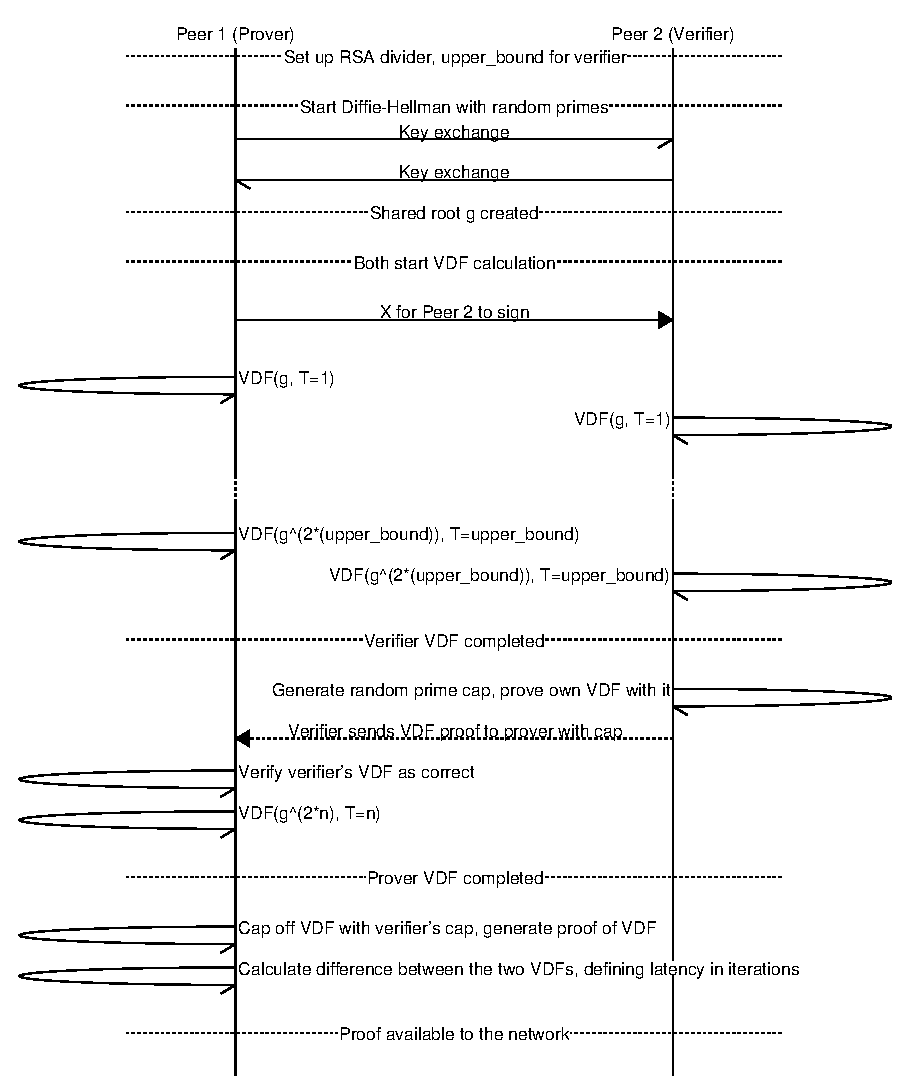
\includegraphics[width=\textwidth]{pictures/pol2_diagram.eps}
	\caption{Protocol Diagram, Proof of Latency}
	\label{PoL Diagram 2}
\end{figure}
Proof of Latency is an interactive public-coin protocol that produces a publicly verifiable non-interactive proof by publishing the parameters with the proof, signed by the participants. The protocol cannot be made non-interactive because of the requirements involved with 
The most important part when calculating any VDF is the setup. If a prover wants to create a valid proof, it needs a previously unknown starting point at first, so that it can prove for certain that it cannot have calculated the VDF in advance. Proof of Latency tackles this problem with a two-way RSA Diffie-Hellman key setup with random ephemeral prime numbers, which is an industry standard to achieve a previously unknown key with large certainty. 

The proof generation removes trust between the two peers by introducing a race between them. The two participants are called the prover and the verifier, although they both are actively proving and verifying their VDFs. The difference here is that they both calculate a VDF and the verifier calculates the difference in iterations between the two.

First the prover and the verifier do a Diffie-Hellman key exchange to construct a previously unknown key. Then, they both start calculating a VDF in parallel. The prover only calculates the VDF up to a predefined threshold, and then sends the proof with a signature back to the verifier. The verifier then stops its own calculation, generates a proof of it, and then calculates the absolute difference between the amount of iterations between its own VDF and the prover's.

Since calculating a VDF is relatively easy for modern processors, a VDF over as little as a few milliseconds of time can be a valid way of measuring latency. Still, without an ASIC chip for calculating VDFs faster than any other available processor, these protocols are also a measurement of processing performance. This might introduce an unfortunate barrier for entry for mobile and IoT devices. The second version of PoL is meant to tackle this problem by creating a performance and latency gradient to the network. The network topology results in a gradient that is defined by geographical location and the similarity in performance. This means that connectedness between mobile and IoT devices is going to be better than between devices that have a huge performance difference.

\section{Attack Vectors}
Since Proof of Latency removes security quarantees by removing randomness from routing, some new attack vectors are introduced. The two versions of the algorithm differ much in terms of security. Proof of Latency is not meant to be a one-stop shop towards a safer network, but rather an add-on to make things more efficient while still keeping security in mind. The following attack vectors are a product of prior knowledge, research and the writer's thought process, and none have been tested out in practice, yet.

\subsection{Advertising Dishonest Peers and Proof Spoofing}
A sybil network participant can spawn an arbitrarily large number of new identities and network peers that are close-by, create multiple Proofs of Latency with them, and only advertise these peers to the rest of the network on their DHT. Two peers can also fake the proof if they co-operate by using VDFs they have already calculated and matched their outputs to be as close as possible. 

This can be mitigated somewhat by requiring peers to renew their proofs regularly, using witnesses or a verifiable source of randomness. Also, trusted computing modules could be used to verify that the software configuration hasn't been changed, removing most of the possibility for side channel attacks against using witnesses.

A way to protect against coordinated proof spoofing is to introduce an unbiased third party to the protocol. Since the soundness of the proof depends largely on the generator and its setup, the proof can be improved by requiring it to be salted by a random input from an unbiased party. How to achieve this? Introduce a salt pool to which a group of PoL witnesses post random salts from which the PoL provers then pick randomly. The witnesses listen for usage of the salts they have generated, and upon receiving the Proof of Latency inspect if their salt has been used or not, and decide to sign or discard the proof based on that.

\subsection{Performance Matching}
Both versions suffer from the same issue, let's call it performance matching, which is a timing attack. Timing attacks are a family of attacks against computer systems called side-channel attacks, which attack the fact that although software is abstract and can be very well fit against any attacks on the software level, outer factors still affect the hardware it runs on. Timing attacks rely on gathering of timing data from the target.~\cite{noauthor_undated-mp} In performance matching, this means connecting to the targeted peer by another protocol or comparing existing proofs of latencies from all peers that have calculated their latency with the target.

Performance matching enables attackers to perform an eclipse attack on low-performance devices by matching the attacker's performance with the targeted mobile device so that it is as close as possible in the difference between iterations in PoL. Now again, if the algorithm had a trusted platform module requirement, or we had an ASIC for repeated squarings, this wouldn't be an issue. This attack could result in a complete network split.

\section{Protecting Against Performance Matching}
\subsection{Hiding Information of VDF Results}
Zero-knowledge proofs could be used to protect against performance matching. If the publicized proof didn't include both the VDF results and iterations, but just included the iteration difference, an attacker would have less info on each peer. This would make attacking more difficult, requiring more queries and PoL runs on average before finding a vulnerable peer.

\subsection{Web of Trust}
There's also a possibility of introducing a web of trust in parallel to PoL to recognize and shut out malicious peers more effectively. An example of such a system is SybilLimit, which adds a construction called trusted routes to DHT based routing.~\cite{Yu2008-xl} I see that trusted routes in conjunction with Proof of Latency would be a great couple. The problem of advertising dishonest peers could also be tackled with a trust based system. Introducing too much trust into the system could also make PoL useless, since there could be a simple ping protocol with a millisecond measurement latency instead.
~
\subsection{Peer Scoring}
Peer scoring is used regularly in P2P networks, 
Proof of Latency serves as a peer scoring metric by itself, and can be used in various ways. To hinder any attacks, peers with the lowest latencies would be kept for a longer time even in the case of the peer not being online, and favoring new ephemeral connections that are farther. 

\subsection{Using a Witness}
A way to make Proof of Latency fully trustless is to introduce an unbiased third party to the protocol. Since the soundness of the proof depends largely on the generator and its setup, the proof can be improved by requiring it to be salted by a random input from an unbiased party. How to achieve this? Introduce a salt pool to which a group of PoL witnesses post random salts from which the PoL provers then pick randomly. The witnesses listen for usage of the salts they have generated, and upon receiving the Proof of Latency inspect if their salt has been used or not, and 

\chapter{Proof of Concept}
\label{Proof of Concept}
To test out Proof of Latency, I made a software proof of concept in Rust. I picked Rust as a programming language because I've wanted to try it out in my own projects for long, and it has some good properties when it comes to cryptography and distributed computing. Since distributed computing or any server program for that matter uses some sort of concurrency to get non-blocking responses to requests they receive, you have a very good chance of running into race conditions with most systems programming languages. When a Rust program has been written in the default "safe" compiler setting, a data race where two or more threads try to access a shared memory resource at the same time is simply impossible to achieve.~\cite{The_Rust_Project_Developers2018-xh} Also, as it is a compiled language without a garbage collector, and with lots of optimization in the compiler, Rust has good baseline performance even when compared to other similarly low level programming languages like Go.~\cite{Howarth2020-zc} Rust has seen a surge of interest in the last few years, and is used in many projects in production, notably in embedded and distributed computing, the former because of Rust's modern build tooling and robustness.

William Borgeaud's blog post~\cite{Borgeaud2019-wk} from November 2019 in particular was the first reference I encountered that described verifiable delay functions in familiar terms to a software engineer like me. The blog post and it's accompanying code~\cite{Borgeaud2019-wk} that also happened to be in Rust helped me bootstrap the project.

First of all, I knew I had to make the VDF run asynchronously, or if possible, in another thread, because it would be one of two VDFs needed in the protocol. There needs to be a separate task for listening to the other party's input, and to make it possible to test locally without networking. For the VDF that is used in Proof of Latency it was also needed that the prover's calculation could be ran indefinitely and ended abruptly by a received "cap" prime number from the verifier. No previous VDF library seemed to have this option, because the difficulty parameter T is usually predetermined in contrast to Proof of Latency.

The code is structured as follows: A runnable binary demo (main.rs) and the reusable library it also uses (lib.rs) resides in the top crate. They both depend on the subcrates "P2P" and "vdf". Here is an example output of Proof of Latency run:
\begin{longlisting}[H]
	\caption{Proof of Latency test run}
	\inputminted
	[
		frame=lines,
		framesep=2mm,
		baselinestretch=1.2,
                breaklines=true,
                fontsize=\footnotesize,
		tabsize=2,
	]
	{text}{./parts/code/samplerun.txt}
	\label{lst:samplerun.txt}
\end{longlisting}

To achieve a better algorithm design, the library itself is described as a state machine, which also helps in thinking of the algorithm in TLA+. Variable names have been converted into more readable non-mathematical forms.
% TODO: Diagram of the state machine, generated by "sm"?

The following is a code example of the threaded evaluation part of a VDF inside proof of latency, containing evaluation stop logic for both the prover and the verifier:
\begin{longlisting}[H]
	\inputminted
	[
		frame=lines,
		framesep=2mm,
		baselinestretch=1.2,
		fontsize=\footnotesize,
		tabsize=2,
	]
	{Rust}{./parts/code/vdfiteration.rs}
        \caption{VDF iteration logic}
	\label{lst:vdfiteration.rs}
\end{longlisting}

The following is a code example of the proof generation of a VDF:
\begin{listing}[H]
	\inputminted
	[
		frame=lines,
		framesep=2mm,
		baselinestretch=1.2,
		fontsize=\footnotesize,
		tabsize=2,
	]
	{Rust}{./parts/code/proofgeneration.rs}
        \caption{VDF proof generation}
	\label{lst:proofgeneration.rs}
\end{listing}

The following is a code example of the verification of a VDF proof:
\begin{listing}[H]
	\inputminted
	[
		frame=lines,
		framesep=2mm,
		baselinestretch=1.2,
		fontsize=\footnotesize,
		tabsize=2,
	]
	{Rust}{./parts/code/verifyvdf.rs}
        \caption{VDF proof verification}
	\label{lst:verifyvdf.rs}
\end{listing}

The proof of concept is made as a library, so that it can be imported in other projects and tinkered with. To make it into a library in addition to a stand-alone binary, I used structs for logical instances of a single VDF, for example. This is mainly to keep program state in instances of these structs, removing possible side effects.

% TODO: TESTS!

\section{Tests}
\subsection{Unit Tests}
To make sure that the VDF calculations worked on arbitrary input by generating a succesfully verifiable proof I made unit tests for the VDF evaluation, proof generation and verification. To further ensure the soundness of the algorithm, I made simulated cases for proof of latency with unit tests with separate, async threads for each execution. Unit tests reside in the same file the program code itself, and the Rust standard library has well enough functionality so that I wasn't forced to use a separate library for assertations\footnote{Checking that a statement holds true or is equal to something}, for example.

In addition to regular unit tests with predefined input, I dabbled in property testing. Property testing is a term that belongs somewhere between fuzzing\footnote{Testing systems against highly randomized and a high volume of input.} and unit tests. Otherwise it functions like regular unit tests, but it adds generated input into the equation. By adding generated, sometimes randomized input, one can check more thoroughly for edge cases. While being effective in recognizing some unexpected bugs, it still has a way to go when compared to formal verification, which is a testing method that aims to define a system with mathematic proofs, verifying that the output should always, apart from hardware issues, be predictable and deterministic.

\subsection{End to End Tests}
To test the whole demo out in a simulated P2P setting I used Protocol Labs' Testground software. It is a tool to simulate a network with thousands of peers on one machine.

\chapter{Future Considerations}
\label{Future Considerations}
If this system was integrated to a blockchain or a publicly verifiable source of randomness for the initial setup, the proofs could be verified by anyone against consensus. Not only this would add trust to the latency measurements, but also speed up initial bootstrapping of the P2P network. When P2P networks eventually grow larger and larger, the network bootstrapping infrastructure needs to be rethought to handle more traffic and be faster in its initialization. By getting introduced to the closest peers possible right at the start the user can experience a more performant network right from the beginning, lowering the barrier for entry by making first impressions better. 

Also, I believe the work is not cryptographically as secure as it could be, and the field is progressing at a mindnumbing pace. Making sure the algorithm is VDF-agnostic would be a logical next step, since the field is still in progress of finding the best possible formulation of a VDF. Quantum computing can render all existing VDF types insufficient, and new VDF types could change the parameter logic fundamentally. The idea behind this thesis is to think of a new creative way of using verifiable delay functions by defining a protocol, and not to necessarily use the most robust cryptography available. 
